\chapter{Dagens pasientsignalsystem ved St. Olavs Hospital}
\label{appendix_dagenssystem}
 
I dette appendikset vil vi beskrive dagens pasientsignalsystem basert på informasjon gitt av Brukermanual for Pasientsignal og Pasientsignalapplikasjon (ref kilde) og brukermanual for Telefoni: Trådløs telefon.

\section{Dagens pasientsignalsystem}
Et signal utløses fra sengerom, fellesrom, stuer, bad ol., for å tilkalle/alarmere pleiepersonell. Det skilles mellom to typer signaler, pasientsignal og hasteanrop, hvor pasientsignal utløses av pasient, mens hasteanrop utløses av pleiepersonell. 
Pasientsignalsystemet er sammensatt av to integrerte systemer, et fast og et trådløst. Det faste systemet, også refererert til som pasientsignalanlegget, består av fastmonterte paneler med trekksnorer og/eller trykknapper: anropspanel \ref{anropspanel}, rompanel \ref{rompanel} og vaktromsapparat \ref{vaktromsapparat}.

\begin{figure}[H]
        \centering
        \begin{subfigure}[b]{0.3\textwidth}
        		\centering
                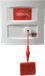
\includegraphics[scale=0.7]{anropspanel.png}
                \caption{Anropspanel}
                \label{anropspanel}
        \end{subfigure}%
        \begin{subfigure}[b]{0.3\textwidth}
        		\centering
                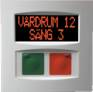
\includegraphics[scale=1.5]{rompanel.jpg}
                \caption{Rompanel}
                \label{rompanel}
        \end{subfigure}
        \begin{subfigure}[b]{0.3\textwidth}
        		\centering
                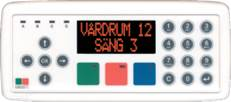
\includegraphics[scale=1]{vaktromsapparat.jpg}
                \caption{Vaktromsapparat}
                \label{vaktromsapparat}
        \end{subfigure}
        \caption{Pasientsignalanlegget}\label{pasientsignalanlegget}
\end{figure}
\noindent
Det finnes to typer anropspanel, et for våtrom og et for vanlig rom. I vanlige sengerom er anropspanelet plassert ved sengen, og har en trykknapp med lysdiode og en trekksnor.
Trykknappen utløser et hasteanrop, mens trekksnoren utløser et pasientsignal.

\noindent
Rompanelet er plassert ved døren til hvert av sengerommene i et sengetun. Det har et display, en grønn og en rød trykknapp med hver sin lysdiode. Grønn knapp trykkes for å markere pleiepersonells tilstedeværelse eller for å avslutte et hasteanrop. Rød knapp trykkes for å utløse pasientsignal, eller et hasteanrop etter at tilstedemarkering er aktivert. Rød knapp kan også holdes inne i 2 sekunder for å utløse hasteanrop, dersom tilstedemarkering ikke er aktivert. 

\noindent
Vaktromsapparatet er sentralt plassert i det åpne landskapet i sengetunet. Det består av et display og flere tall- og tegntaster. Displayet indikerer stedangivelse for et pasientsignal, hasteanrop og tilstedemarkerte rom. Pasientsignaler og hasteanrop er signalisert med rød tekst, mens tilstedemarkering er vist ved grønn tekst. Tastene brukes for å programmere apparatet.

\noindent
Disse er videre tilkoblet det trådløse systemet, som består av følgende IKT-komponenter: pasientsignalapplikasjon \ref{pasientapplikasjon}, trådløs telefonenhet \ref{telefon} og pasientterminal \ref{pasientterminal}.

\begin{figure}[H]
        \centering
        \begin{subfigure}[b]{0.35\textwidth}
        		\centering
                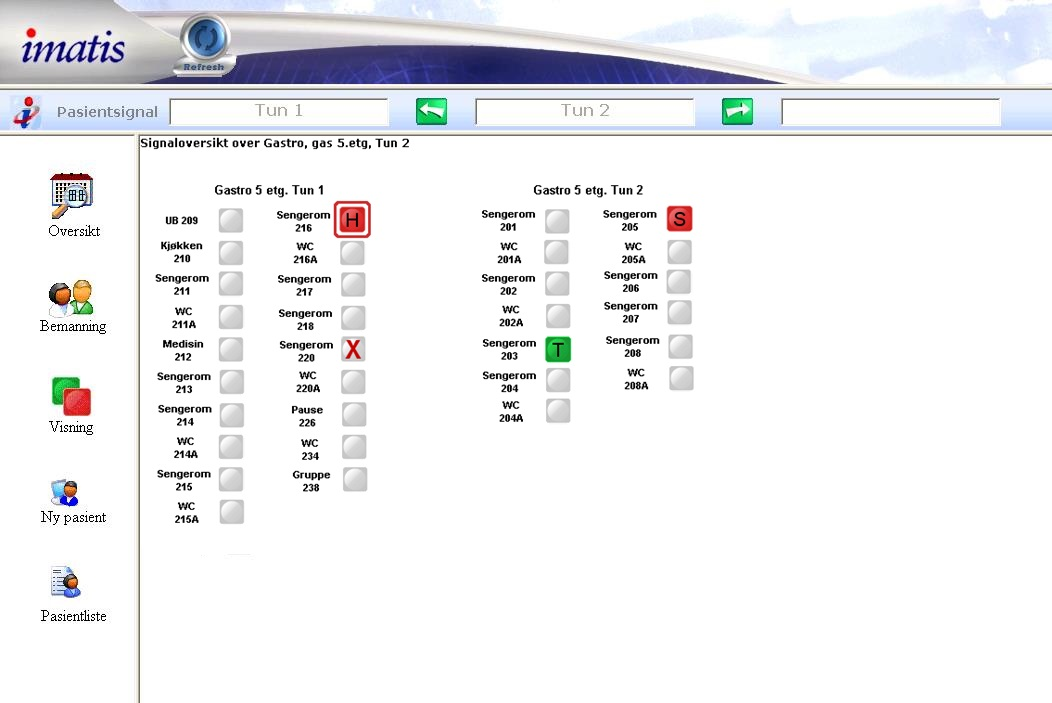
\includegraphics[scale=0.2]{pasientapplikasjon.jpg}
                \caption{Pasientsignalapplikasjon}
                \label{pasientapplikasjon}
        \end{subfigure}%
        \begin{subfigure}[b]{0.35\textwidth}
        		\centering
                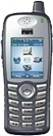
\includegraphics[scale=1]{telefon.jpg}
                \caption{Trådløs telefonenhet}
                \label{telefon}
        \end{subfigure}
        \begin{subfigure}[b]{0.25\textwidth}
        		\centering
                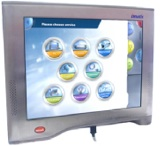
\includegraphics[scale=0.4]{pasientterminal.jpg}
                \caption{Pasientterminal}
                \label{pasientterminal}
        \end{subfigure}
        \caption{Det trådløse systemet}\label{dettradlosesystemet}
\end{figure}
\noindent
Pasientsignalapplikasjonen kjører på hvert sengetuns PC, 24 timer i døgnet, hver dag. Applikasjonen tilbyr i hovedsak fem funksjoner: (1) oversikt, (2) bemanning, (3) visning, (4) registrering av ny pasient og (5) en pasientliste. Vi vil her utdype funksjonene bemanning og visning, da disse er av mest relevans for vår oppgave.  

\noindent
Bemanningsplanen, vist i figur \ref{bemanningsplan}, knytter tilgjengelig pleiepersonell til rommene ved et sengetun. Pasientsignalene vil dermed sendes til riktig mottaker på bakgrunn av bemanningsplanen. For å anvende denne funksjonaliteten må adgangskort plasseres i kortleser tilkoblet PC'en. For hvert rom vil det normalt tilknyttes en primærsykepleier og en disponibel sykepleier.
\begin{figure}[H]
\centering
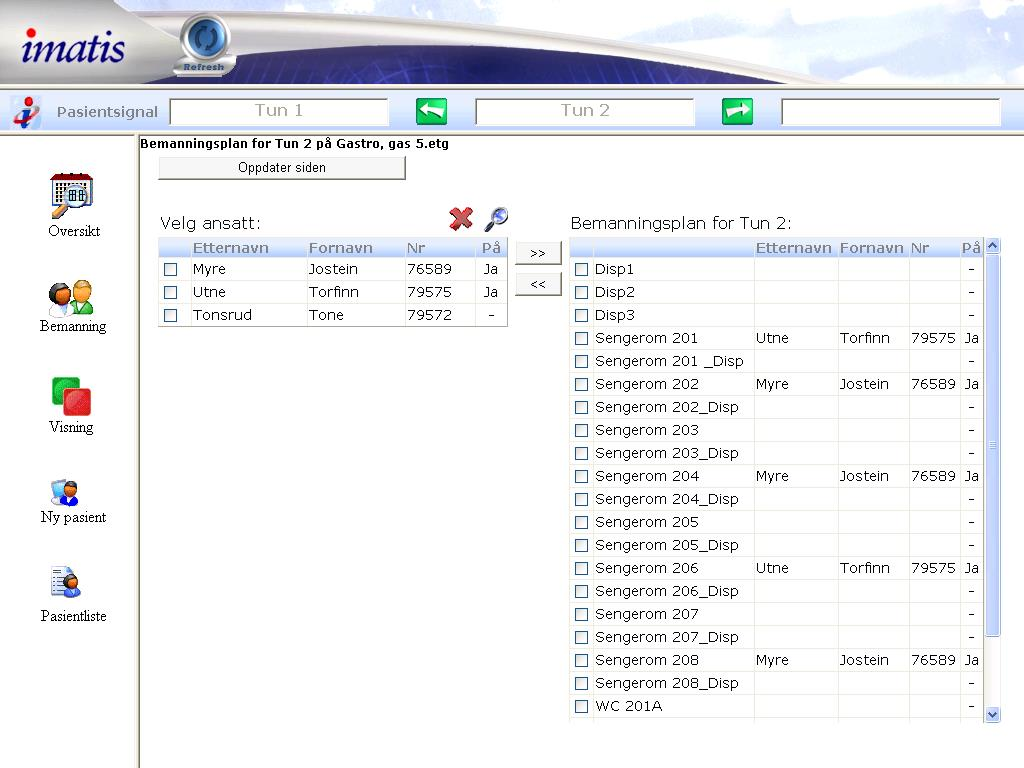
\includegraphics[scale=0.4]{bemanningsplan.jpg}
\caption{Bemanningsplan}
\label{bemanningsplan}
\end{figure}
\noindent
Funksjonen visning, vist i figur \ref{visning}, viser en oversikt over pasientsignalanlegget ved gjeldende sengetun, her vist som Gastro 5. etasje, tun en og to. Grønn T markerer at pleiepersonell har trykket på den grønne knappen på rompanelet i det gjeldende sengerommet, og tilsynelatende er tilstede. Dette er nødvendigvis ikke riktig, da pleiepersonell kan glemme å trykke av den grønne knappen da de forlater rommet. Rød S signaliserer et pasientsignal, mens innrammet rød H signaliserer et hasteanrop. Rødt kryss varsler feil i systemet.
\begin{figure}[H]
\centering
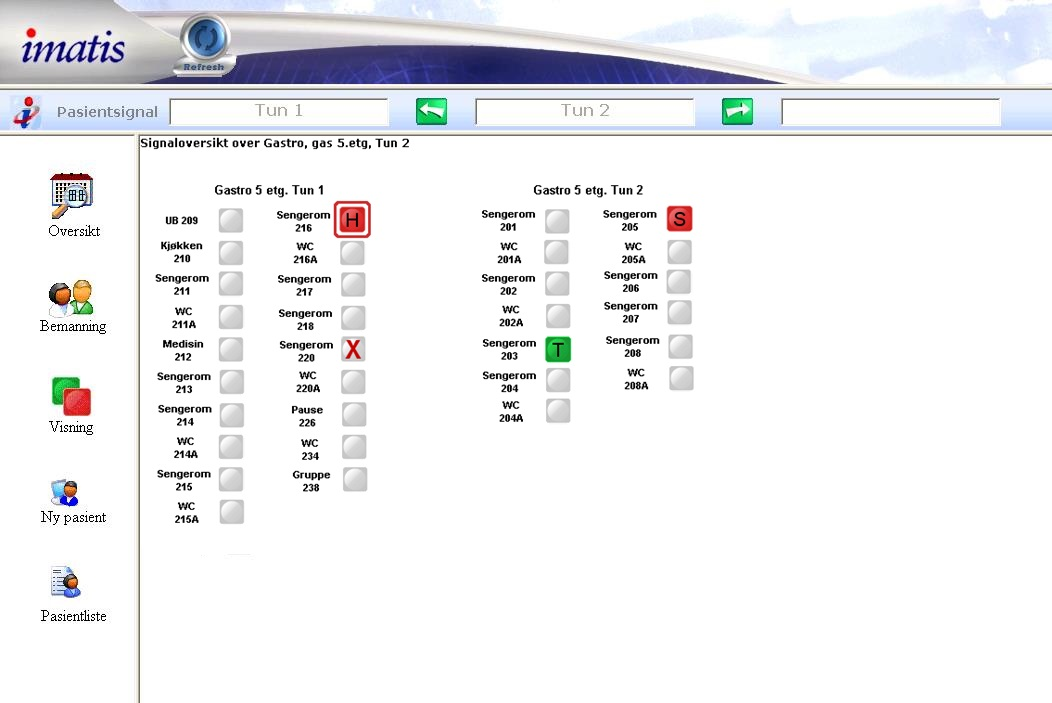
\includegraphics[scale=0.4]{pasientapplikasjon.jpg}
\caption{Visning}
\label{visning}
\end{figure}
\noindent
De trådløse telefonenhetene inngår i det IP-baserte telefonisystemet ved St. Olavs Hospital, og er av typen Cisco Wireless IP Phone 7921G. I tillegg til å tilby basisfunksjoner, som å ringe og sende tekstmeldinger, støtter de tjenester for alarmering. Pleiepersonell logger seg på telefonene for å motta pasientsignal og hasteanrop.

\noindent
Pasienterminalen inneholder en rekke funksjoner som pasienten kan benytte seg av, deriblant TV, radio, telefon, internett, spill og trykknapp for pasientsignal. Den røde knappen under skjermen benyttes for å utløse pasientsignal, og denne fungerer uavhengig av om terminalen er skrudd på eller ikke.

\noindent
Nå som de ulike komponentenes funksjon og hensikt er blitt utdypet, vil vi forklare hvordan de fungerer sammen. 

\begin{figure}[H]
\centering
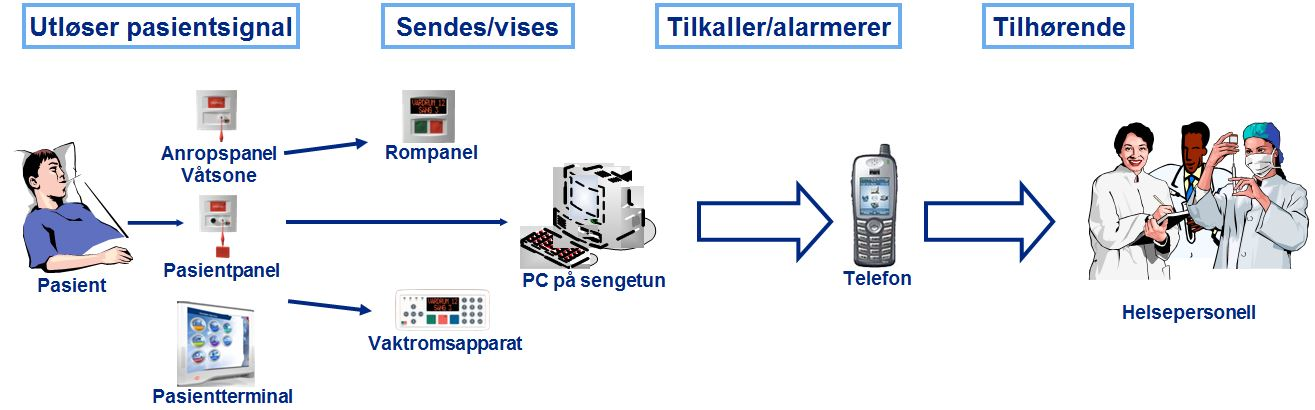
\includegraphics[scale=0.4]{alarmprosess.jpg}
\caption{Pasientsignal}
\label{alarmprosess}
\end{figure}












